% !TeX root = ../main.tex

\section{Decision Making Under Vagueness and
Uncertainty}

\subsection{Aspects of Belief and Uncertainty in Opinions}

\subsubsection{Sharp Belief Mass}

\begin{definition}
    \emph{(Sharp Belief Mass)} Let $\mathbb{X}$ be a domain with hyperdomain $\mathcal{R}(\mathbb{X})$
and variable $X$. Given an opinion $\omega_X$, the sharp belief mass of value $x \in \mathcal{R}(\mathbb{X})$ is the function $\mathbf{b}^{\mathrm{S}}_X : \mathcal{R}(\mathbb{X}) \rightarrow [0, 1]$ expressed as
    \begin{equation}
        \text{Sharp belief mass: } \mathbf{b}^{\mathrm{S}}_X = \sum\limits_{x_i \subseteq x} \mathbf{b}_X(x_i)\text{, }\forall x \in \mathcal{R}(\mathbb{X})\text{.}
    \end{equation}
\end{definition}

\begin{definition}
    \emph{(Total Sharp Belief Mass)} Let $\mathbb{X}$ be a domain with variable $X$, and let $\omega_X$ be an opinions on $\mathbb{X}$. The total sharp belief mass contained in the opinion $\omega_X$ is the function $\mathbf{b}^{\mathrm{TS}}_X : \mathbb{X} \rightarrow [0, 1]$ expressed as
    \begin{equation}
        \text{Total Sharp belief mass: } b^{\mathrm{TS}}_X = \sum\limits_{x_i \subseteq \mathbb{X}} \mathbf{b}_X(x_i)\text{.}
    \end{equation}
\end{definition}

The total belief sharpness denoted b S X is simply the sum of all belief masses
assigned to singletons

\subsubsection{Vague Belief Mass}

The vague belief mass on a value $\mathbf{x} \in \mathcal{R}(\mathbb{X})$ is defined as the weighted sum of belief masses on the composite values of which $x$ is a member, where the weights are determined by the base rate distribution.

\begin{definition}
    \emph{(Vague Belief Mass)} Let $\mathbb{X}$ be a domain with hyperdomain $\mathcal{R}(\mathbb{X})$ and composite set $\mathcal{C}(\mathbb{X})$. Given an
opinion $\omega_X$, the vague belief mass on $x \in \mathcal{R}(\mathbb{X})$ is the function $\mathbf{b}^\mathrm{V}_X : \mathcal{R}(\mathbb{X}) \rightarrow [0, 1]$:
    \begin{equation}
        \text{Vague belief mass: } \mathbf{b}^{\mathrm{V}}_X(x) = \sum\limits_{\substack{x_i \in \mathcal{C}(\mathbb{X}) \\ x_i \nsubseteq x}} \mathbf{a}_X(x | x_i) \mathbf{b}_X(x_i) \text{, } \forall x \in \mathcal{R}(\mathbb{X}) \text{.}
    \end{equation}
\end{definition}

\begin{definition}
    \emph{(Total Vague Belief Mass)} Let $\mathbb{X}$ be a domain with variable $X$, and
let $\omega_X$ be an opinions on $\mathbb{X}$. The total vagueness contained in the opinion $\omega_X$ is the
function $\mathbb{b}^{\mathrm{TV}}_X : \mathcal{C}(\mathbb{X}) \rightarrow [0, 1]$ expressed as:
    \begin{equation}
        \text{Total vague belief mass: } b^{\mathrm{TV}}_X = \sum\limits_{x \in \mathcal{C}(\mathbb{X})} \mathrm{b}_X(x) \text{.}
    \end{equation}
\end{definition}

\subsubsection{Dirichlet Visualization of Opinion Vagueness}

Example: The singletons and composite values of $\mathcal{R}(\mathbb{X})$ are listed below.

\begin{equation}
    \left\{\begin{array}{lll}
        \text{Domain:}        & \mathbb{X}              & = \{x_1, x_2, x_3\} \text{, } \\
        \text{Hyperdomain:}   & \mathcal{R}(\mathbb{X}) & = \{x_1, x_2, x_3, x_4, x_5, x_6\} \text{,} \\
        \text{Composite set:} & \mathcal{R}(\mathbb{X}) & = \{x_4, x_5, x_6\} \text{,}
    \end{array}\right. \text{where }
    \left\{\begin{array}{l}
        x_4 = \{x_1, x_2\} \text{,} \\
        x_5 = \{x_1, x_3\} \text{,} \\
        x_6 = \{x_2, x_3\} \text{.} \\
    \end{array}\right.
\end{equation}

\begin{equation}
    \begin{array}{l}
        \text{Belief mass distribution} \\
        \left\{\begin{array}{ll}
            \mathbf{b}_X(x_6) & = 0.8 \text{,} \\
            u_X               & = 0.2 \text{.}
        \end{array}\right.
    \end{array} \quad
    \begin{array}{l}
        \text{Base rate distribution} \\
        \left\{\begin{array}{l}
            \mathbf{a}_X(x_1) = 0.33 \text{,} \\
            \mathbf{a}_X(x_2) = 0.33 \text{,} \\
            \mathbf{a}_X(x_3) = 0.33 \text{.} \\
        \end{array}\right.
    \end{array}
\end{equation}

\def\arraystretch{1.5}
\begin{equation*}
    \begin{array}{rl}
         \mathbf{P}_X(x_1) = & \sum\limits_{x_i \in \mathcal{R}(\mathbb{X})} \mathbf{a}_X(x_1 | x_i) \mathbf{b}_X(x_i) + \mathbf{a}_X(x_1) u_X \\
                           = & \dfrac{\mathbf{a}_X(\{x_1\} \cap \{x_2, x_3\})}{\mathbf{a}_X(\{x_2, x_3\})} \mathbf{b}_X(x_6) + \mathbf{a}_X(x_1) u_X \\
                           = & 0 + 0.33 \cdot 0.2 \\
                           = & 0.066
    \end{array}
\end{equation*}

\begin{equation*}
    \begin{array}{rl}
        \mathbf{P}_X(x_2) = & \sum\limits_{x_i \in \mathcal{R}(\mathbb{X})} \mathbf{a}_X(x_2 | x_i) \mathbf{b}_X(x_i) + \mathbf{a}_X(x_1) u_X \\
                          = & \dfrac{\mathbf{a}_X(\{x_2\} \cap \{x_2, x_3\})}{\mathbf{a}_X(\{x_2, x_3\})} \mathbf{b}_X(x_6) + \mathbf{a}_X(x_1) u_X \\
                          = & \dfrac{0.33}{0.66} \cdot 0.8 + 0.33 \cdot 0.2 \\
                          = & 0.467
    \end{array}
\end{equation*}

\begin{equation*}
    \mathbf{P}_X(x_3) = 0.467
\end{equation*}

\begin{equation*}
    \begin{array}{rl}
        \mathbf{b}^{\mathrm{V}}_X(x_1) = & \sum\limits_{\substack{x_i \in \mathcal{C}(\mathbb{X}) \\ x_i \nsubseteq x}} \mathbf{a}_X(x_1 | x_i) \mathbf{b}_X(x_i) \\
                                       = & \dfrac{\mathbf{a}_X(\{x_1\} \cap \{x_2, x_3\})}{\mathbf{a}_X(\{x_2, x_3\})} \mathbf{b}_X(x_6) \\
                                       = & 0 \cdot 0.8 \\
                                       = & 0
    \end{array}
\end{equation*}

\begin{equation*}
    \begin{array}{rl}
        \mathbf{b}^{\mathrm{V}}_X(x_2) = & \sum\limits_{\substack{x_i \in \mathcal{C}(\mathbb{X}) \\ x_i \nsubseteq x}} \mathbf{a}_X(x_2 | x_i) \mathbf{b}_X(x_i) \\
                                       = & \dfrac{\mathbf{a}_X(\{x_2\} \cap \{x_2, x_3\})}{\mathbf{a}_X(\{x_2, x_3\})} \mathbf{b}_X(x_6) \\
                                       = & \dfrac{0.33}{0.66} \cdot 0.8 \\
                                       = & 0.4
    \end{array}
\end{equation*}

\begin{equation*}
    \mathbf{b}^{\mathrm{V}_X}(x_3) = 0.4
\end{equation*}

\def\arraystretch{1}
\begin{equation}
    \begin{array}{l}
        \text{Projected probability distribution} \\
        \left\{\begin{array}{l}
            \mathbf{P}_X(x_1) = 0.066 \text{,} \\
            \mathbf{P}_X(x_2) = 0.467 \text{,} \\
            \mathbf{P}_X(x_3) = 0.467 \text{.}
        \end{array}\right.
    \end{array} \quad
    \begin{array}{l}
        \text{Vague belief mass} \\
        \left\{\begin{array}{l}
            \mathbf{b}^{\mathrm{V}}_X(x_1) = 0.0 \text{,} \\
            \mathbf{b}^{\mathrm{V}}_X(x_2) = 0.4 \text{,} \\
            \mathbf{b}^{\mathrm{V}}_X(x_3) = 0.4 \text{.}
        \end{array}\right.
    \end{array}
\end{equation}

Figure 4.2 from the book shows the hyper-Dirichlet PDF for this vague opinion.

\subsubsection{Focal Uncertainty Mass}

\begin{definition}
    \emph{(Focal Uncertainty Mass)} Let $\mathbb{X}$ be a domain and $\mathcal{R}(\mathbb{X})$ denote its
hyperdomain. Given an opinion $\omega_X$, the focal uncertainty mass of an value $x \in \mathcal{R}(\mathbb{X})$
is computed with the function $\mathbf{u}^{\mathrm{F}}_X : \mathcal{R}(\mathbb{X}) \rightarrow [0, 1]$ defined as
    \begin{equation}
        \text{Focal uncertainty mass: } \mathbf{u}^{\mathrm{F}}_X(x) = \mathbf{a}_X(x) u_X \text{.}
    \end{equation}
\end{definition}

\subsection{Mass-sum}

\subsubsection{Mass-Sum of a Value}

The sum of sharp belief mass, vague belief mass and focal uncertainty mass of a
value $x$ is equal to the value's projected probability, expressed as

\begin{equation}
    \mathbf{b}^{\mathrm{S}}_X(x) + \mathbf{b}^{\mathrm{V}}_X(x) + \mathbf{b}^{\mathrm{F}}_X(x) = \mathbf{P}_X(x)
\end{equation}

\begin{definition}
    \emph{(Mass-Sum)} Let $\mathbb{X}$ be a domain with hyperdomain $\mathcal{R}(\mathbb{X})$, and assume that the opinion $\omega_X$ is specified. Consider a value $x \in \mathcal{R}(\mathbb{X})$ with sharp belief mass $\mathbf{b}^{\mathrm{S}}_X(x)$, vague belief mass $\mathbf{b}^{\mathrm{V}}_X(x)$ and focal uncertainty mass $\mathbf{b}^{\mathrm{F}}_X(x)$. The mass-sum function of value $x$ is the triplet denoted $\mathbf{M}_X(x)$ expressed as
    \begin{equation}
        \text{Mass-sum of x: } \mathbf{M}_X(x) = \left( \mathbf{b}^{\mathrm{S}}_X(x), \mathbf{b}^{\mathrm{V}}_X(x), \mathbf{b}^{\mathrm{F}}_X(x) \right)
    \end{equation}
\end{definition}

In order to visualize it, consider the ternary domain $\mathbb{X} = \{x_1, x_2, x_3\}$:

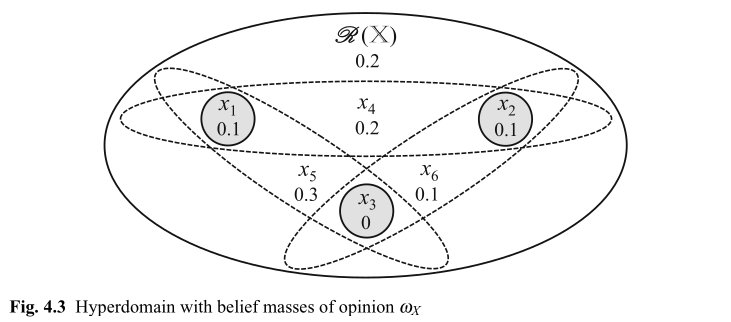
\includegraphics[width=\linewidth]{images/fig.4.3.png}

The following table shows the projected probability of each value of $x$.

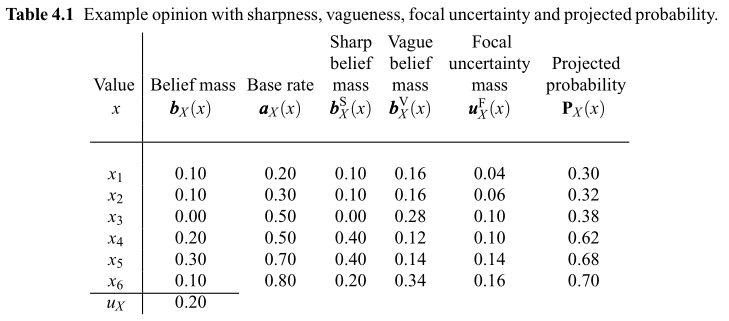
\includegraphics[width=\linewidth]{images/tab.4.1.png}

The \emph{mass-sums} can be easily visualized by a mass sum diagram. Since opinions in higher
dimension can’t be visualized by a simplex, a mass sum diagram makes easier to compare
opinions and appreciate its nature.

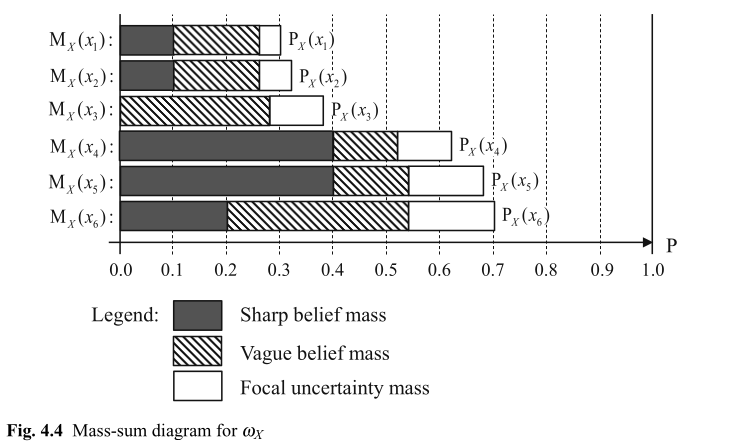
\includegraphics[width=\linewidth]{images/fig.4.4.png}

Although $x_3$ has the highest projected probability, it has no sharp belief mass. Differentiating
between those parts of an opinion might be important for decision making and will be showed
bellow.

\subsubsection{Total Mass-Sum}

The belief mass of an opinion as a whole can be decomposed into sharp belief mass
which provides distinctive support for singletons, and vague belief mass which provides vague support for singletons. These two belief masses are then complementary
to the uncertainty mass. For any opinion $\omega_X$ it can be verified that Eq.(\ref{eq:total_mass_sum}) holds:
\begin{equation}\label{eq:total_mass_sum}
    b^{\mathrm{TS}}_X + b^{\mathrm{TV}}_X + u_X = 1
\end{equation}

\begin{definition}
    \emph{(Total Mass-Sum)} Let $\mathbb{X}$ be a domain with hyperdomain $\mathcal{R}(\mathbb{X})$, and
assume that the opinion $\omega_X$ is specified. The total sharp belief mass $b^{\mathrm{TS}}_X$, total vague
belief mass $b^{\mathrm{TV}}_X$ and uncertainty mass $u_X$ can be combined as a triplet, which is then called the total mass-sum, denoted $\mathrm{M}^{\mathrm{T}}_X$ and expressed as
    \begin{equation}
        \text{Total mass sum: } \mathrm{M}^{\mathrm{T}}_X = \left( b^{\mathrm{TS}}_X, b^{\mathrm{TV}}_X, u_X \right)
    \end{equation}
\end{definition}

The total mass-sum of opinion $\omega_X$ is illustrated bellow:

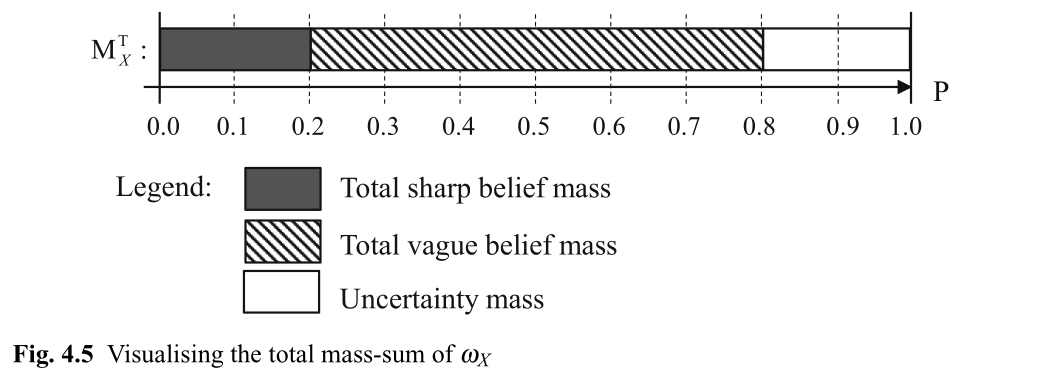
\includegraphics[width=\linewidth]{images/fig.4.5.png}

\subsection{Utility and Normalization}

Assume a random variable $X$ with an associated projected probability distribution
$\mathbf{P}_X$. Utility is typically associated with outcomes of a random variable, in the sense that for each outcome $x$ there is an associated utility $\bm{\lambda}_X(x)$ expressed on some scale
such as monetary value, which can be positive or negative. Given utility $\bm{\lambda}_X(x)$ in
case of outcome $x$, then the expected utility for $x$ is
\begin{equation}
    \text{Expected utility: } \mathbf{L}_X(x) = \bm{\lambda}_X(x) \mathbf{P}_X(x) \text{.}
\end{equation}

Total expected utility for the variable $X$ is then
\begin{equation}
    \text{Total expected utility: } \mathrm{L}^{\mathrm{T}}_X(x) = \sum\limits_{x \in \mathbb{X}} \bm{\lambda}_X(x) \mathbf{P}_X(x) \text{.}
\end{equation}

\begin{definition}
    \emph{(Utility-Normalised Probability Vector)} Assume a random variable $X$ with an associated projected probability distribution $\mathbf{P}_X$ and a utility vector
$\bm{\lambda}_X$, which together produce the expected utility distribution $\mathbf{L}_X$. Let $\lambda^+$ denote the
greatest absolute utility from $\bm{\lambda}_X$ and from other relevant utility vectors to be considered for comparing different options. The utility-normalised probability vector produced by $\mathbf{P}_X$, $\bm{\lambda}_X$ and $\lambda^+$ is expressed as
    \begin{equation}
        \mathbf{P}^{\mathrm{N}}_X(x) = \dfrac{\mathbf{L}_X(x)}{\lambda^+} = \dfrac{\bm{\lambda} \mathbf{P}_X(x)}{\lambda^+} \text{, } \forall x \in \mathbb{X} \text{.}
    \end{equation}
\end{definition}

\begin{definition}
    \emph{(Utility-Normalised Masses)} Assume a random variable $X$ with a
projected probability distribution $\mathbf{P}_X$. Let $\mathbf{b}^{\mathrm{S}}_X(x)$ denote the sharp belief mass of $x$, let
$\mathbf{b}^{\mathrm{V}}_X(x)$ denote the vague belief mass of $x$, and let $\mathbf{u}^{\mathrm{F}}_X(x)$ denote the focal uncertainty
mass of $x$. Assume the utility vector $\bm{\lambda}_X$, as well as $\lambda^+$, the greatest absolute utility
from $\rm{\lambda}_X$ and from other relevant utility vectors to be considered for comparing
different options. The utility-normalised masses are expressed as
    \begin{equation}
        \text{Utility-normalised sharp belief mass: } \mathbf{b}^{\mathrm{NS}}_X(x) = \dfrac{\rm{\lambda}_X(x) \mathbf{b}^{\mathrm{S}_X(x)}}{\lambda^+} \text{, } \forall x \in \mathbb{X}
    \end{equation}
    \begin{equation}
        \text{Utility-normalised vague belief mass: } \mathbf{b}^{\mathrm{NV}}_X(x) = \dfrac{\rm{\lambda}_X(x) \mathbf{b}^{\mathrm{V}_X(x)}}{\lambda^+} \text{, } \forall x \in \mathbb{X}
    \end{equation}
    \begin{equation}
        \text{Utility-normalised focal uncertainty mass: } \mathbf{u}^{\mathrm{NF}}_X(x) = \dfrac{\rm{\lambda}_X(x) \mathbf{u}^{\mathrm{F}_X(x)}}{\lambda^+} \text{, } \forall x \in \mathbb{X}
    \end{equation}
\end{definition}

There is a additivity property on belief masses:
\begin{equation}
    \text{Utility-normalized probability: } \mathbf{b}^{\mathrm{NS}}_X(x) + \mathbf{b}^{\mathrm{NV}}_X(x) + \mathbf{u}^{\mathrm{NF}}_X(x) = \mathbf{P}^{\mathrm{N}}_X(x) \text{.}
\end{equation}

\begin{definition}
    \emph{(Utility-Normalised Mass-Sum)} Let $\mathbb{X}$ be a domain with hyperdomain $\mathcal{R}(\mathbb{X})$, and assume that the opinion $\omega_X$ is specified. Also assume that a
utility vector $\lambda_X$ is specified. Consider a value $x \in \mathcal{R}(\mathbb{X})$ with the utility normalised
    masses $\mathbf{b}^{\mathrm{NS}}_X(x)$, $\mathbf{b}^{\mathrm{NV}}_X(x)$ and $\mathbf{u}^{\mathrm{NF}}_X(x)$. The utility-normalised mass-sum function of $x$
is the triplet denoted $\mathbf{M}^{\mathrm{N}}_X(x)$ expressed as
    \begin{equation}
        \text{Utility-normalised mass-sum: } \mathbf{M}^{\mathrm{N}}_X(x) = \left( \mathbf{b}^{\mathrm{NS}}_X(x), \mathbf{b}^{\mathrm{NV}}_X(x), \mathbf{u}^{\mathrm{NF}}_X(x) \right)
    \end{equation}
\end{definition}

\subsection{Decision Criteria}

When deciding using opinions in subjective logic, the analyst should decide according to a
priority scale defined by the author in the following flow chart:

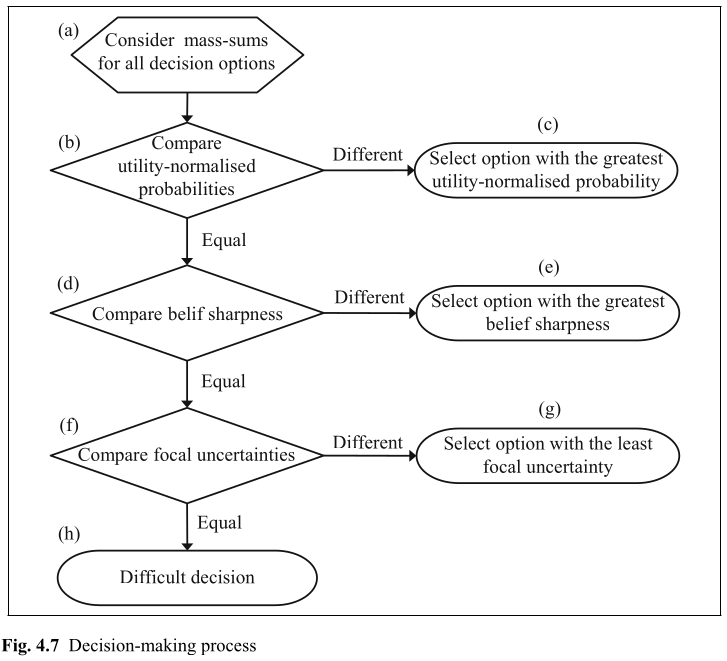
\includegraphics[width=\linewidth]{images/fig.4.7.png}

Thus, dividing our opinion in different parts provided us a better way to decide upon uncertainty, since we can now differentiate where the belief came from.

\subsection{The Ellsberg Paradox}